\chapter{Reducción de datos con Python}
\setcounter{ipythcntr}{0}

Para realizar las tareas básicas de reducción de datos astronómicos usando Python se utiliza el módulo llamado <<\pynorm{ccdproc}>>. Este módulo es una herramienta poderosa diseñada para la reducción y el procesamiento de datos de imágenes CCD. Está desarrollado como parte del ecosistema de <<\pynorm{astropy}>> y proporciona una serie de funciones y clases para manejar tareas comunes en el preprocesamiento de datos astronómicos, como la calibración de imágenes, la corrección de bias, la corrección de flat-field, y la combinación de imágenes. Primero revisaremos el módulo astropy.

\section{El paquete Astropy}
Astropy es un paquete diseñado específicamente para la astronomía y la astrofísica. Cuenta con muchas funciones y módulos, pero nosotros revisaremos algunos de los más utilizados y que nos serán de ayuda para comprender el funcionamiento de \pynorm{ccdproc}. Para instalar \pynorm{astropy}, si es que no lo tienes aún, es suficiente con escribir \bashbold{pip install astropy} en una terminal. 

Algunos de los módulos más populares dentro del ecosistema de astropy son \pynorm{units}, \pynorm{Coordinates}, y \pynorm{fits}. A continuación realizaremos algunas tareas básicas con estos módulos.

\subsection{El módulo astropy.units}
El módulo <<\pynorm{astropy.units}>> permite trabajar con unidades físicas tales como los kilogramos, metros, segundos y cualquiera de sus múltiplos, submúltiplos y además hace posible transformar entre diferentes unidades equivalentes de otros sistemas de medición. 

Primero debemos importarlo:
\begin{pyin}
import astropy.units as u
\end{pyin}

Ahora podemos definir una variable que tenga unidades de distancia. Por ejemplo, podemos asignarle unidades de kilopársec:

\begin{pyin}[]
#- Distancia en kilopársec
distance = 1 * u.kpc
distance
\end{pyin}
\begin{pyout}
<Quantity 1. kpc>
\end{pyout}

Como se ve en la celda de código anterior, se crea una <<cantidad>> al multiplicar cualquier variable numérica por una unidad definida en \pynorm{astropy}. En este caso, el kilopársec se obtiene con <<\pynorm{u.kpc}>>. Si ahora queremos saber a cuántos metros equivale un kilopársec, entonces podemos usar la función <<\pynorm{u.to()}>> de la siguiente manera:

\begin{pyin}[]
#- Convertir a metros
distance.to(u.m)
\end{pyin}
\begin{pyout}
<Quantity 3.08567758e+19 m>
\end{pyout}

Existe otra forma de utilizar la función \pynorm{u.to()}, que es un poco más flexible. Para ilustrarlo, intentemos convertir la variable \pynorm{distance} a varias unidades de distancia, tales como los centímetros, metros, kilómetros, años luz, pársec, nanómetros y unidades astronómicas. Una forma de hacerlo es la siguiente:

\begin{pyin}
distance_units = ['cm', 'm', 'km', 'lyr', 'pc', 'nm', 'au']

#- Distancia equivalente en varias unidades
print(f'{distance} es equivalente a:\n=========================')

for unit in distance_units:
    print( distance.to(u.Unit(unit)) )  
\end{pyin}
\begin{pyprint}
1.0 kpc es equivalente a:
=========================
3.0856775814913673e+21 cm
3.085677581491367e+19 m
3.085677581491367e+16 km
3261.5637771674333 lyr
1000.0 pc
3.085677581491367e+28 nm
206264806.24709633 AU
\end{pyprint}

Por supuesto que se pueden utilizar unidades derivadas, tales como las de la velocidad ($ \mathrm{m/s} $, por ejemplo) o las de la fuerza ($ \mathrm{N \equiv kg~ m~ s^{-2}} $). Para esto usamos los operadores de multiplicación y división según sea el caso. Específicamente, para definir cantidades con unidades de velocidad:

\begin{pyin}
velocity = 60 * u.km / u.h
velocity
\end{pyin}
\begin{pyout}
<Quantity 60. km / h>
\end{pyout}

Obteniendo su equivalente en $ \mathbb{m/s} $:

\begin{pyin}
velocity.to(u.m/u.s)
\end{pyin}
\begin{pyout}
<Quantity 16.66666667 m / s>
\end{pyout}

\subsection{Trabajando con tablas}
Con astropy se pueden leer tablas casi en cualquier formato. Un formato muy popular en astronomía son los archivos con extensión fits (\textbf{F}lexible \textbf{I}mage \textbf{T}ransport \textbf{S}ystem). Una de las formas de leer este tipo de archivos es usando la función \pynorm{Table()} del módulo \pynorm{astropy.table}. Las imágenes CCD se almacenan en archivos \norbash{.fits}. Sin embargo, no es posible leerlas con \pynorm{Table()}. Afortunadamente, existen más opciones. 

Para poder trabajar con imágenes \norbash{.fits} provenientes de archivos CCD, se puede utilizar el módulo \pynorm{fits} que está dentro de \pynorm{astropy.io}. Toma como ejemplo las imágenes disponibles en este enlace de Google drive: \url{https://drive.google.com/drive/folders/1TxopD_fIa1ZHplm_SH0Gvhe663psuJn-?usp=sharing}.

El enlace contiene una carpeta organizada de la siguiente manera: hay un directorio llamado \norbash{bias}, otro llamado \norbash{flats}, otro llamado \norbash{object} y uno llamado \norbash{stds}. Los directorios \norbash{bias} y \norbash{flat} contienen las imágenes bias y flat, respectivamente. El directorio \norbash{object} contiene las imágenes del objeto de interés, también llamadas <<\emph{science images}>> o imágenes de ciencia. El directorio \norbash{stds} contiene imágenes de una estrella estándar, que no usaremos por el momento. 

Recomiendo que extraigas el contenido de la carpeta en tu mismo directorio de trabajo donde utilizas los Notebooks de Jupyter para que puedas acceder a sus datos de manera más simple y con las rutas especificadas en el Notebook llamado <<Astropy-package>>. 

Primero establecemos las rutas a las imágenes:
\begin{pyin}[]
#- Ruta a la ubicación de los datos
bias_image = 'OB0001/bias/0002611406-20200712-OSIRIS-OsirisBias1.fits'
flat_image = 'OB0001/flat/0002615401-20200712-OSIRIS-OsirisSkyFlat1.fits'
object_image = 'OB0001/object/0002611437-20200712-OSIRIS-OsirisBroadBandImage1.fits'  
\end{pyin}

Para leer estas imágenes con el módulo \pynorm{fits}, se hace de la siguiente manera:

\begin{pyin}[]
#- Leyendo la imagen con astropy
bias_data   = fits.open(bias_image)[0]
flat_data   = fits.open(flat_image)[0]
object_data = fits.open(object_image)[0]
\end{pyin}

Debes tener en cuenta que las instrucciones anteriores generarán errores si no guardaste los datos en tu directorio actual de trabajo. Si en cualquier momento ocurre un error de compilación, siempre revisa el mensaje de error. Como hemos visto en ocasiones anteriores, Python brinda mucha información en sus mensajes de errores para que puedas corregirlos. 

Puedes verificar la información contenida en cada imagen aplicando el atributo \pynorm{header}. Por ejemplo para la imagen bias:

\begin{pyin}
bias_data.header
\end{pyin}
\begin{pyprint}
SIMPLE  =                    T / Fits standard                                  
BITPIX  =                   16 / Bits per pixel                                 
NAXIS   =                    2 / Number of axes                                 
NAXIS1  =                 1049 / Axis length                                    
NAXIS2  =                 2051 / Axis length                                    
EXTEND  =                    F / File may contain extensions                    
BSCALE  =           1.000000E0 / REAL = TAPE*BSCALE + BZERO                     
BZERO   =           3.276800E4 /                                                
ORIGIN  = 'NOAO-IRAF FITS Image Kernel July 2003' / FITS file originator        
DATE    = '2021-10-07T01:52:03' / Date FITS file was generated                  
IRAF-TLM= '2021-10-07T01:52:03' / Time of last modification                     
OBJECT  = 'BIAS    '           / Name of the object observed                    
ORIGFILE= 'Jul12_204354.fits'  / Filename                                       
INSTRUME= 'OSIRIS  '           / Instrument Name                                
DETECTOR= 'E2V CCD44_82_BI'    / Detectors Model                                
DETSIZE = '[1:4096,1:4102]'    / Maximum Imaging Pixel Area                     
DATE-OBS= '2020-07-12T20:43:39.592' / Time when starts the first exposure (in fr
ELAPSED = '22.969  '           / Total elapsed time from start to end (s)       
...       
\end{pyprint}

Para acceder a la imagen se necesita del atributo \pynorm{data}:
\begin{pyin}
bias_data.data
\end{pyin}
\begin{pyprint}
array([[1039, 1137, 1156, ..., 1203,   29,  881],
       [1037, 1133, 1171, ..., 1192,   28,  892],
       [1044, 1135, 1170, ..., 1204,   29,  896],
       ...,
       [1069, 1160, 1184, ..., 1224,   28,  897],
       [1062, 1157, 1180, ..., 1231,   29,  892],
       [1068, 1160, 1188, ..., 1221, 1224,  102]], dtype=uint16)
\end{pyprint}

Como puedes darte cuenta, la imagen CCD es un arreglo de numpy bidimensional. Para poder visualizarlo, necesitamos usar la función \pynorm{imshow()}. Sin embargo, los datos tienen una cantidad bastante grande de pixeles:

\begin{pyin}
bias_data.data.size
\end{pyin}
\begin{pyout}
2151499
\end{pyout}

Dada la cantidad de pixeles, es necesario aplicar una función para escalar la imagen. Para eso utilizamos la función \norbash{show_image} que está definida dentro del archivo llamado \norbash{show_image.py} en el directorio de Notebooks. Importamos esa función y la utilizamos:

\begin{pyin}
from show_image import show_image

show_image(bias_data.data, cmap='gray')
plt.title('Imagen BIAS')
plt.show()
\end{pyin}

\noindent
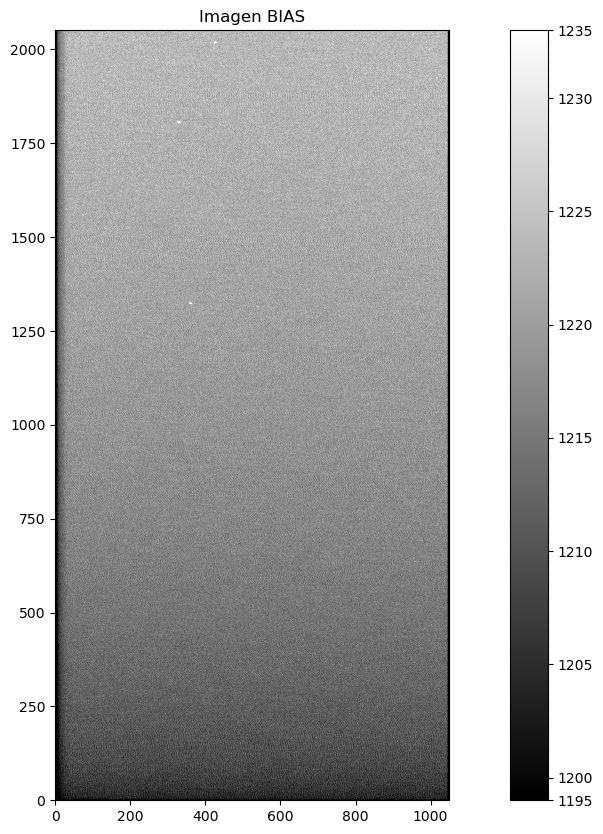
\includegraphics[width=0.4\textwidth]{figures/binary_bias_example.png}

De igual manera podemos visualizar la imagen de campo plano:
\begin{pyin}
show_image(flat_data.data, cmap='gray')
plt.title('Imagen FLAT')
plt.show()
\end{pyin}

\noindent
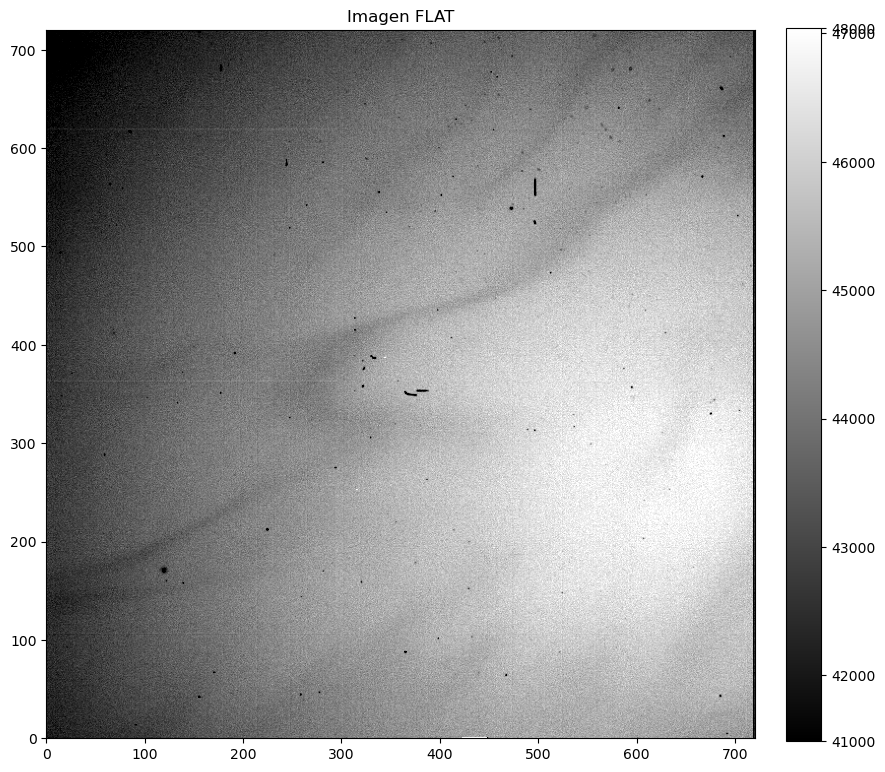
\includegraphics[width=0.5\textwidth]{figures/binary_flat_example.png}

Y también la imagen del objeto:
\begin{pyin}
show_image(object_data.data, cmap='gray')
plt.title('Imagen del objeto')
plt.show()
\end{pyin}

\noindent
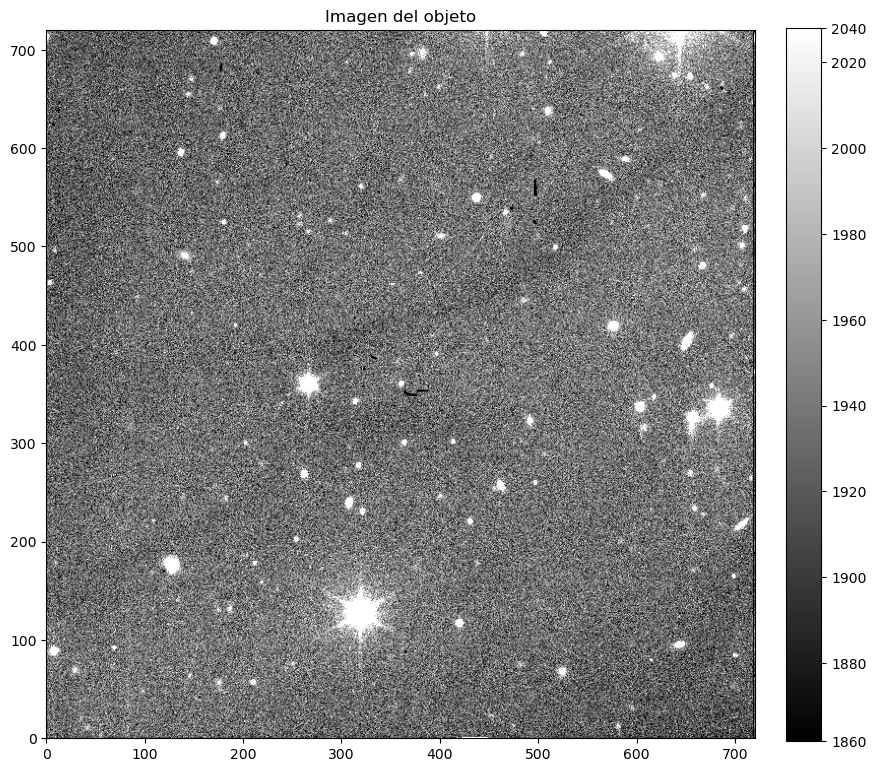
\includegraphics[width=0.5\textwidth]{figures/binary_object_example.png}

\subsection{Un ejemplo un poco realista}
Ahora revisemos un ejemplo bastante sencillo sobre el proceso de reducir una imagen CCD. Para eso vamos a generar una imagen sintética, o en otras palabras, a simular una imagen astronómica. Utilizaremos las funciones definidas dentro del módulo \pynorm{image_sim} para generar una imagen de bias, una flat y una de dark current. Primero importamos el módulo:

\begin{pyin}
import image_sim as imsim
\end{pyin}

Comenzamos definiendo los parámetros de cada imagen:
\begin{pyin}
stars_exposure = 30.0
dark_exposure = 60.0
dark = 0.1
sky_counts = 20
bias_level = 1100
read_noise = 700
max_stars_counts = 2000
\end{pyin}

Generamos las imágenes de bias, dark current y flat:

\begin{pyin}
bias_with_noise = (imsim.bias(image, bias_level, realistic=True) + 
                   imsim.read_noise(image, read_noise))

dark_frame_with_noise = (imsim.bias(image,bias_level,realistic=True) + 
                         imsim.dark_current(image, dark, dark_exposure, hot_pixels=True) +
                         imsim.read_noise(image, read_noise))

flat = imsim.sensitivity_variations(image)
\end{pyin}

Creamos la imagen con estrellas y ruido:
\begin{pyin}
realistic_stars = (imsim.stars(image,50,max_counts=max_stars_counts) +
                   imsim.dark_current(image, dark, stars_exposure,  hot_pixels=True) +
                   imsim.bias(image, bias_level, realistic=True) +
                   imsim.read_noise(image, read_noise)
                  )
\end{pyin}

Ya que las imágenes simuladas para bias y dark frames no tienen el mismo tiempo de exposición, se necesita hacer una escalación:

\begin{pyin}
scaled_dark_current = stars_exposure * (dark_frame_with_noise - bias_with_noise) / dark_exposure
\end{pyin}

Y este es nuestro primer intento de reducir una imagen astronómica:

\begin{pyin}
calibrated_stars = (realistic_stars - bias_with_noise - scaled_dark_current) / flat
\end{pyin}

Visualizar la imagen tal vez no nos brinde mucha información sobre si la imagen mejoró o no. Pero podemos observar el histograma de cuentas. Para lograrlo, importamos el siguiente módulo:

\begin{pyin}
from astropy.visualization import hist
\end{pyin}

Ahora graficamos el histograma para la imagen simulada y su correspondiente calibración:

\begin{pyin}
plt.figure(figsize=(9, 9))
hist(calibrated_stars.flatten(), bins='freedman', label='Imagen calibrada', alpha=0.5)
hist(stars_with_noise.flatten(), bins='freedman', label='Imagen cruda', alpha=0.5)
plt.legend()
plt.grid()
plt.xlabel('Nivel de cuentas en la imagen')
plt.ylabel('Número de pixeles con esas cuentas') 
\end{pyin}

\noindent
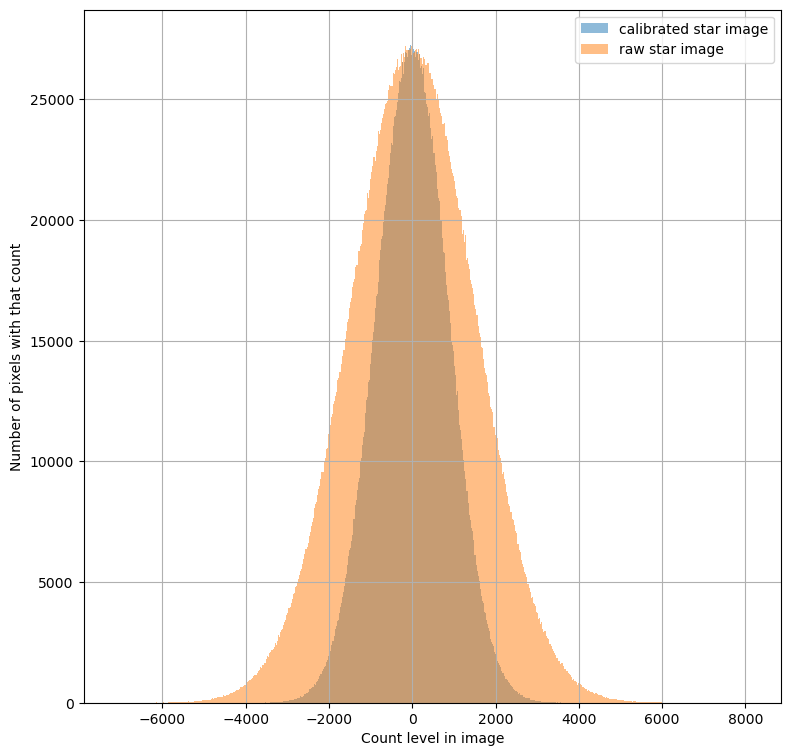
\includegraphics[width=0.7\textwidth]{figures/counts_hist_simulated.png}

En la gráfica anterior, el ruido de la imagen CCD está representado por el espesor de la distribución del histograma. Vemos que el espesor de la imagen calibrada es menor al de la imagen sin calibrar. En otras palabras, hemos logrado reducir el ruido de la imagen CCD. En las siguientes clases veremos cómo realizar una calibración de manera correcta. 
